\chapter{Text Classification}

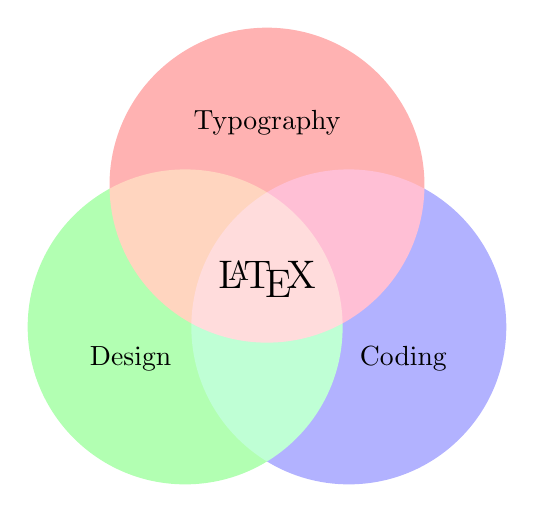
\begin{tikzpicture}
  \begin{scope}[blend group = soft light]
    \fill[red!30!white]   ( 90:1.2) circle (2);
    \fill[green!30!white] (210:1.2) circle (2);
    \fill[blue!30!white]  (330:1.2) circle (2);
  \end{scope}
  \node at ( 90:2)    {Typography};
  \node at ( 210:2)   {Design};
  \node at ( 330:2)   {Coding};
  \node [font=\Large] {\LaTeX};
\end{tikzpicture}

The process of~filtering data we described in the~first chapter is known as {\bf text classification}.
\citet{AggZhai12} describe text classification as follows.
We have a~set of~training records~$\mathcal{D} = \left\{X_1, \ldots, X_N\right\}$ and each record is labeled with one~of the~class labels indexed by~$\left\{1,\ldots, k\right\}$.
Every record consists of~attributes which contain some~information about it.

The~training set is used for building a~{\bf classification model}. Classification model is a~mapping between a~record and a~class label.
In~this document we will take into account only \emph{hard version} of~classification which explicitly maps one and only one label to each record.  

\section{Text Classification Process}

\todoA{diagram:}
\begin{code}
obtaining dataset
-> preprocessing {extraction} -> feature selection
 ^^^^^^^^^^^^^^^^^^^^^^^^^^^^^^^^^^^^^^^^^^^^^^^^^^^^^^
    		feature engineering

-> training -> evaluation
\end{code}
\begin{figure}
	blah blah
\label{cls_process}
\end{figure}

JOIN 2.1 and 2.3, reorganize thorough spec

To get a model and measure performance, we will follow the process of building a classifier as depicted in~\ref{cls_process}.

Subsequently, we have a~set of testing records.
These records are classified by our built models and used for comparing their performance.
More on exact evaluation in \autoref{chap:eval}.

To be consistent with machine learning terminology, we will refer to a~record as {\bf an~instance} and to an~attribute as {\bf a~feature}.

\citet{Song14} 

\section{Thorough Specification of Data}

Let us define our task again with the~introduced terminology.
Each review is an~instance and file \texttt{review.json} contains an~instance per line.
Because the raw data cannot be directly used as features, we have to extract our features first.
An~example of such a~feature is the~number of words in a~review, which is calculated from the~review's text.
More on feature creation is discussed in \autoref{chap:fea}.
Business information will be only used indirectly to drop reviews coming for unreliable sources.

\section{Overview of the Classification Process}

As mentioned above, we will describe {\it feature engineering} in \autoref{chap:fea}.
Firstly, we will introduce several common approaches to creating features and also discuss possibilities of features tailored exactly for our problem.
Secondly, we will talk about {\it feature selection}, that is a process of identifying and eliminating unhelpful features for both classification and computational performance reasons.

The general concept of classifiers will be introduced in \autoref{chap:clsgen}, individual classifiers then in \autoref{chap:clscon}.
Common metrics used for evaluating performance of our classifier are discussed in \autoref{chap:eval}.

Last three chapters are then left for the architecture of the software developed (\autoref{chap:arch}), demonstration of conducted experiments (\autoref{chap:exp}) and final discussion (\autoref{chap:concl}).
